\section{Auswertung}
\subsection{Energiekalibration}
Die Energiekalibration wird anhand der Vermessung eines $^{152}\symup{Eu}$-Spektrums (Abb. \ref{fig:eu_spectrum}) durchgeführt.
Die Messdaten werden mit Python 3.7.3 und den Biblitheken \textit{numpy}, \textit{scipy} und \textit{uncertainties} ausgewertet.
Ausgleichsrechnungen erfolgen mit \\\textit{scipy.optimize.curve\_fit}.
Über eine Peak-Picking-Funktion werden die größten Peaks in den Daten ausfindig gemacht und sind in Tabelle \ref{tab:eu_peaks} notiert.
\begin{figure}[h!]
  \centering
  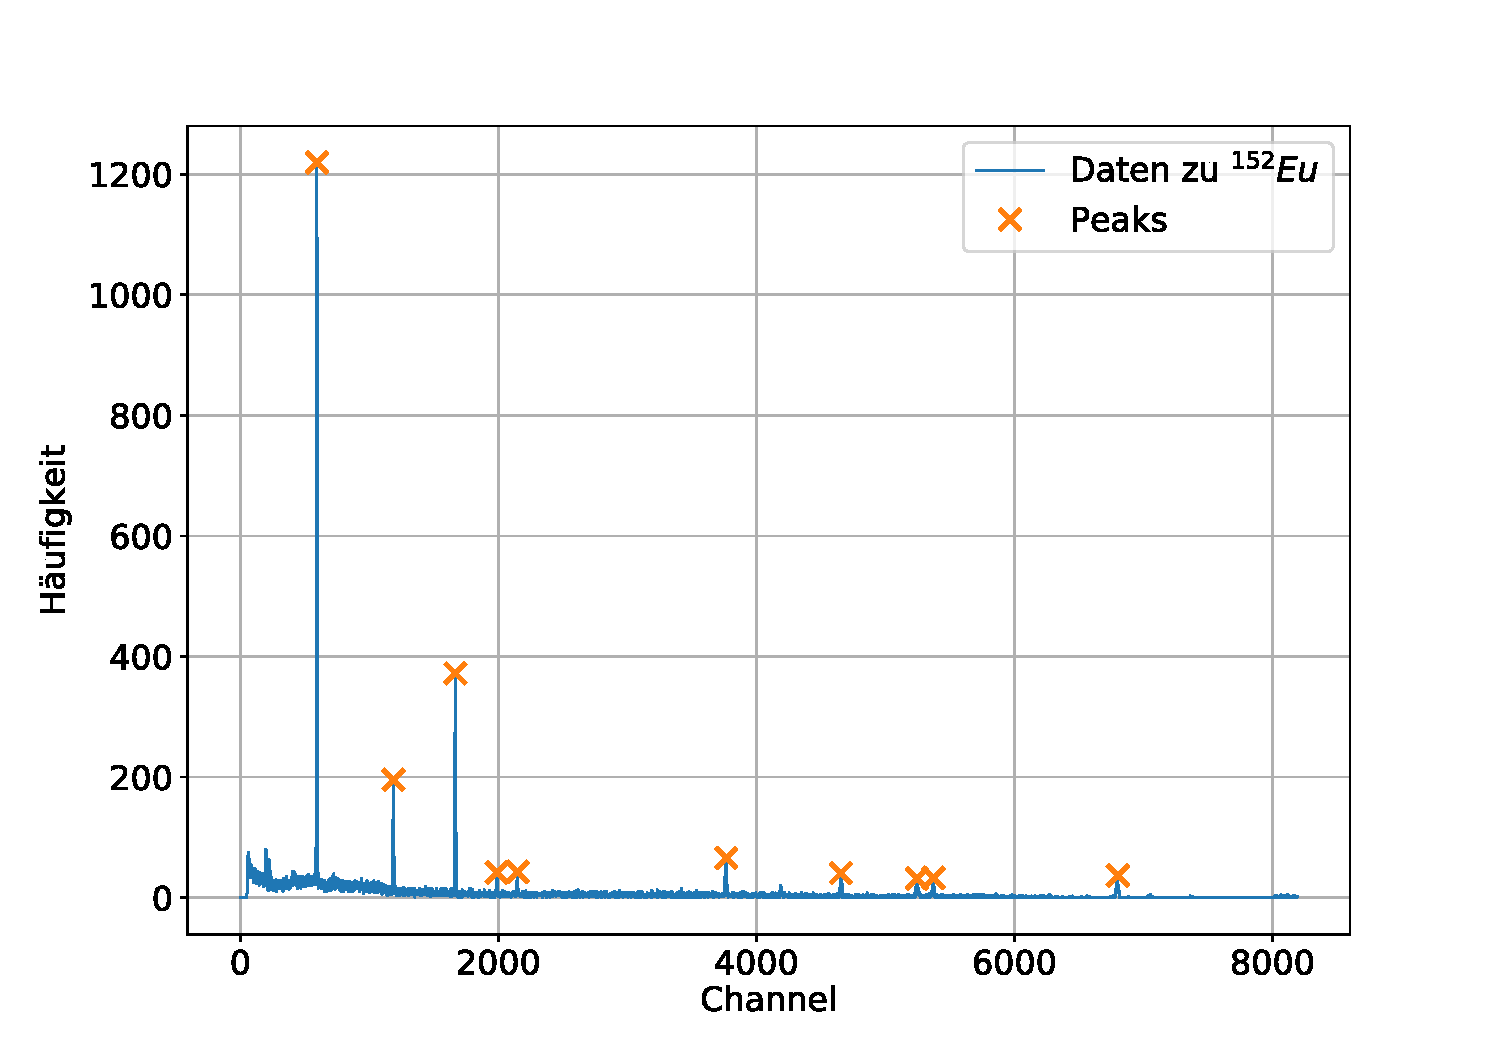
\includegraphics[width=0.8\textwidth]{content/images/spektrum_europium.pdf}
  \caption{Das aufgenommene Spektrum über $T=\SI{2134}{s}$ von $^{152}\symup{Eu}$ mit markierten Peaks. Dargestellt ist die Zählrate gegen den zugehörigen Channel des MCA.}
  \label{fig:eu_spectrum}
\end{figure}
Zum $\gamma$-Zerfall des $^{152}\symup{Eu}$ werden Literaturwerte bezüglich der Emissionsenergien und der Emissionswahrscheinlichkeiten recherchiert \cite{nucleide}.
Dabei werden zunächst die Emissionsenergien mit mindestens $\SI{1}{\%}$ Emissionswahrscheinlichkeit rausgesucht.
Diese sind in Tabelle \ref{tab:eu_peaks} aufgeführt.
\begin{table}[h!]
  \centering
  \caption{Parameter zu allen vermessenen Peaks des $^{152}\symup{Eu}$-Spektrums.}
  \label{tab:eu_peaks}
  \begin{tabular}{ r  r  r  r  r  r  }
    \bottomrule
            Peak & Channel(Peak)  & Counts  &  $E_{\gamma}$ / keV \cite{nucleide} & rel. Channel                                       & rel. Energie  \\ % & $a$                              &      $\mu$                         & $\sigma$                         & $b$                              \\
                 &                &         &                                     & $\frac{\text{Channel}}{\text{Channel(Peak 9)}}$    & $\frac{E_{\gamma}}{E_{\gamma}\text{(Peak 9)}}$ \\ % & $a$                              &      $\mu$                         & $\sigma$                         & $b$                              \\
    \midrule
            0    &  594           &  1219   &  $\SI{121.7817}{\nothing}$          & 0,087                                              & 0,087 \\
            1    &  1187          &  196    &  $\SI{244.6974}{\nothing}$          & 0,175                                              & 0,174 \\
            2    &  1667          &  372    &  $\SI{344.2785}{\nothing}$          & 0,245                                              & 0,245 \\
            3    &  1988          &  42     &  $\SI{411.1165}{\nothing}$          & 0,292                                              & 0,292 \\
            4    &  2149          &  43     &  $\SI{ 443.965}{\nothing}$          & 0,316                                              & 0,315 \\
            5    &  3765          &  66     &  $\SI{778.9045}{\nothing}$          & 0,554                                              & 0,553 \\
            6    &  4655          &  41     &  $\SI{ 964.079}{\nothing}$          & 0,685                                              & 0,685 \\
            7    &  5245          &  32     &  $\SI{1085.837}{\nothing}$          & 0,771                                              & 0,771 \\
            8    &  5371          &  33     &  $\SI{1112.076}{\nothing}$          & 0,790                                              & 0,790 \\
            9    &  6801          &  37     &  $\SI{1408.013}{\nothing}$          & 1,0                                                & 1,0 \\
    \toprule
  \end{tabular}
\end{table}
%                                &  \scriptsize{$\sfrac{mN}{sm}{a}$}            &  \scriptsize{$\sfrac{mN}{m}{a}$}          &  \scriptsize{$\sfrac{mN}{m}{a}$} &  \scriptsize{$\sfrac{mN}{m}{a}$} & \scriptsize{$\sfrac{mN}{m}{a}$} \\ \hline \hline
%    \rowcolor{Lightgray} \multicolumn{7}{|c|}{Referenzen}\\ \hline
%        \multirow{2}{*}{\ce{C3F8}}  & 1  & $\SI{ 1.3396 \pm 0.0202 e-3}{\nothing}{a}$  &  $\SI{ -0.5415 \pm 0.0558 }{\nothing} $  &  $\SI{ 0.00 }{\nothing}{a}$      &  $\SI{ 5.72 }{\nothing}{a}$   & $\SI{ 5.72 }{\nothing}{a}$    \\

Zur Kalibration werden die jeweiligen Daten auf den zugehörigen Wert des letzten sichtbaren Peaks normiert.
Entsprechend werden folgende Rechnungen ausgeführt:
\begin{align*}
	\text{rel. Energie } && E_{\text{rel.}} 				&& = && \frac{ E_{\text{Peak}} }{ E (\text{Peak=9}) } \\
	\text{rel. Channel } && \text{Channel}_{\text{rel.}} 	&& = && \frac{ \text{Channel} }{ \text{Channel} (\text{Peak=9}) }. \\
\end{align*}
Die relativen Größen sind in Abbildung \ref{fig:eu_kalibration} gegen die Counts aufgetragen.
Die drei Emissionsenergien, die im gemessenen Spektrum nicht als Peak ersichtlich sind und auch die geringsten Emissionswahrscheinlichkeiten aufweisen, werden aus den Daten der Literaturwerte entfernt.
\begin{figure}[h!]
  \centering
  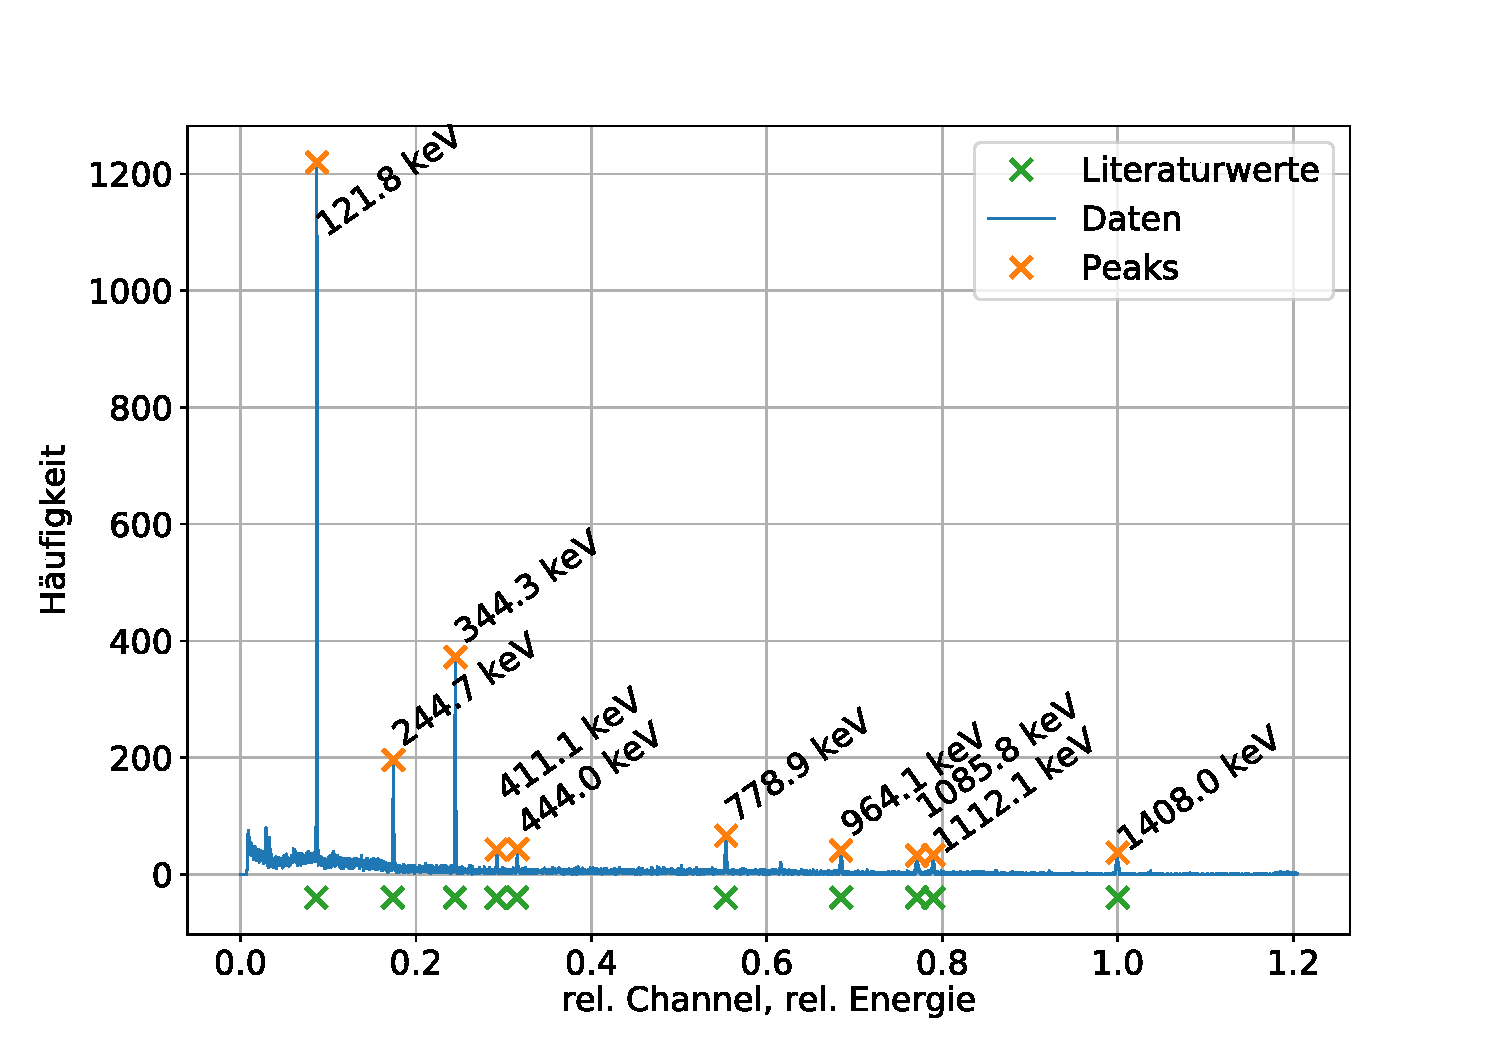
\includegraphics[width=0.8\textwidth]{content/images/spektrum_europium_kali.pdf}
  \caption{Die relativen Größen $E_{\text{rel.}}$ und $\text{Channel}_{\text{rel.}}$, normiert auf den letzten sichtbaren Peak des $^{152}\symup{Eu}$-Spektrums, sind gegen die zugehörigen Counts aufgetragen.
  Die Peaks lassen sich nun den Spektrallinien des $^{152}\symup{Eu}$ zuordnen.}
  \label{fig:eu_kalibration}
\end{figure}
Anschließend werden die zugeordneten Energien der Peaks gegen die Channel der Peaks geplottet (Abbildung \ref{fig:kalibration}) und es wird eine lineare Regression der Form
\begin{equation}
	E = m \cdot \text{Channel} + n
\end{equation}
durchgeführt.
Als Parameter der Regression ergeben sich über \textit{curve\_fit}:
\begin{align*}
	m = \SI{0.20726(4)}{\kilo \electronvolt \per Channel}, && n = \SI{-1.22(17)}{\kilo \electronvolt}.
\end{align*}
\begin{figure}[h!]
  \centering
  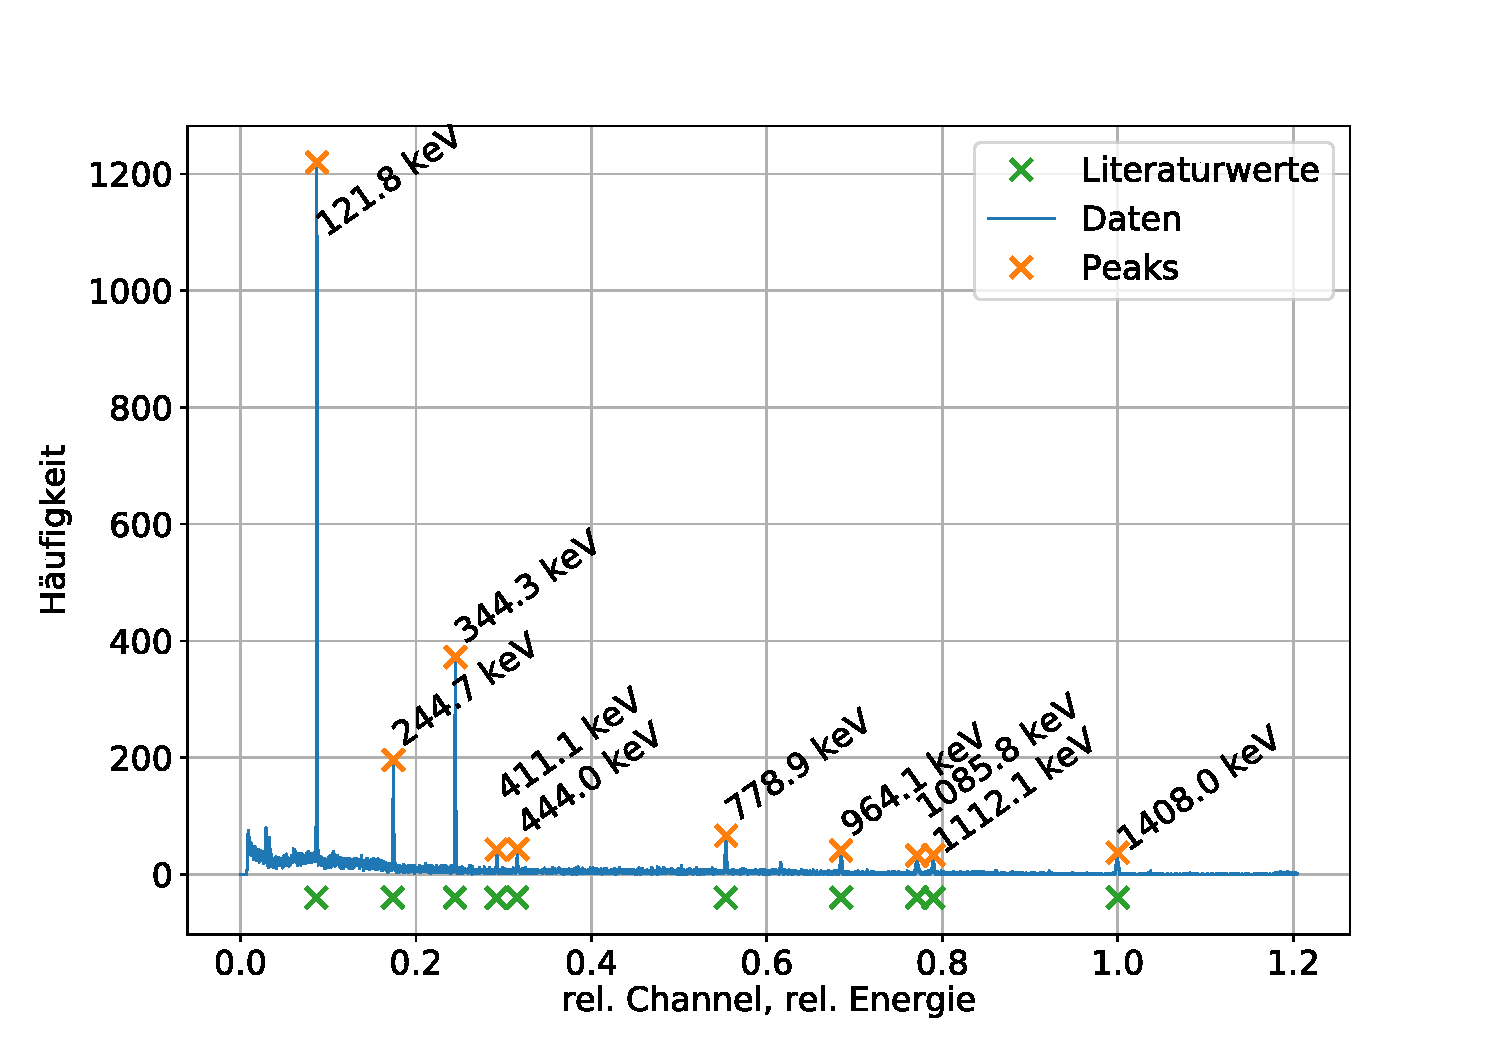
\includegraphics[width=0.8\textwidth]{content/images/spektrum_europium_kali.pdf}
  \caption{Ausgleichsrechnung über den Zusammenhang der Channel des MCA und der Energien der $\gamma$-Teilchen.}
  \label{fig:kalibration}
\end{figure}


%\begin{itemize}
%	\item Spektrum geplottet, Counts gegen Channel
%	\item Errorbars?
%	\item Peaks finden lassen, Peaks markiert
%	\item Literaturwerte Energien rausgesucht mit mind. 1\% Emissionswahrscheinlichkeit (Quelle %http://www.nucleide.org/DDEP_WG/Nuclides/Eu-152_tables.pdf 2019-12-11, 22:35)
%	\item Spektrallinien $E$ normiert mit dem größten Wert der Energie: $\frac{E}{max(E)}$
%	\item Channel normiert mit dem letzten Peak $\frac{channel}{max(channel)}$
%	\item Daten mit normierter x-Achse geplottet: norm(E)-0-Diagramm, norm(channel)-Count-Diagramm
%	\item Nicht vorhandene Spektrallinien aus E und doppelte aus Peaks entfernt
%	\item Peak-Channel gegen Energien geplottet, Fit:
%\end{itemize}
%\begin{equation*}
%	E = m \cdot \text{Channel} + n
%\end{equation*}
%\begin{align*}
%	m = \SI{0.20726(4)}{\kilo \electronvolt \per Channel} && n = \SI{-1.22(17)}{\kilo \electronvolt}
%\end{align*}




\FloatBarrier
\subsection{Vollenergienachweiswahrscheinlichkeit}
Zur Bestimmung der Vollenergienachweiswahrscheinlichkeit $Q$ (engl.: \textit{efficiency}) des Detektors wird zunächst die Aktivität der Probe ausgerechnet.
Zwischen dem angegebenen Herstellungsdatum (01.10.2000) \cite{anleitung} der $^{152}\symup{Eu}$-Probe und dem Versuchstag (09.12.2019) sind $t = \SI{605484000 (54000)}{s}$ vergangen.
Die Halbwertszeit des Isotops beträgt $T_{\sfrac{1}{2}} = \SI{426.7 (5) e+06}{s}$ \cite{nucleide}.
Mit der Anfangsaktivität $A_{0} = \SI{4130 (60)}{Bq}$ ergibt sich über
\begin{equation}
	A = A_{0} \exp{\left( - \frac{\ln{(2)}}{T_{\sfrac{1}{2}}} t \right)} = \SI{1545(29)}{\per \second}
	\label{result:aktivität}
\end{equation}
die aktuelle Aktivität der Probe.
Weiterhin wird der eingenommene Raumwinkel des Detektors benötigt.
Dabei wird der Raumwinkel über die Geometrie eines Kegels berechnet:
\begin{align*}
	\frac{r}{h} = \tan{( \varphi / 2 )} \Leftrightarrow \varphi = 2 \arctan{(\frac{r}{h})} \\
	\frac{\Omega}{4 \pi} = \sin^2{\frac{\varphi}{2 \cdot 4}} =  \sin^2{ \left( \frac{1}{4} \arctan{(r/h)} \right)} = \SI{0.0069}{sr}.
	\label{result:raumwinkel}
\end{align*}
Die eingesetzten Größen für den Radius der Detektoroberfläche und Höhe des Kegels sind $r = \SI{22.5e-03}{m}$ und $h = \SI{80e-03}{m}$.
Die gesamte Messzeit des $^{152}\symup{Eu}$-Spektrums beträgt $T=\SI{2134}{s}$.
Damit kann nun $Q$ wie folgt berechnet werden:
\begin{equation}
	Q = \frac{4 \pi}{\Omega} \frac{N_{\text{Peakinhalt}}}{ A T P_{E_{\gamma}}}.
\end{equation}
$P_{E_{\gamma}}$ ist hier die Emissionswahrscheinlichkeit einer $\gamma$-Energie \cite{nucleide}.
Der Parameter $N_{\text{Peakinhalt}}$ beschreibt nun die gesamte Zahl der Counts, die sich in einem Peak befindet.
Zur Berechnung der Peakinhalte werden die Peaks einzeln betrachtet und die Messdaten passend zu der erwarteten Gaußverteilung eines Peaks abgeschnitten (vgl. Abb. \ref{fig:einzelnergaussfit_0}).
\begin{figure}[h!]
  \centering
  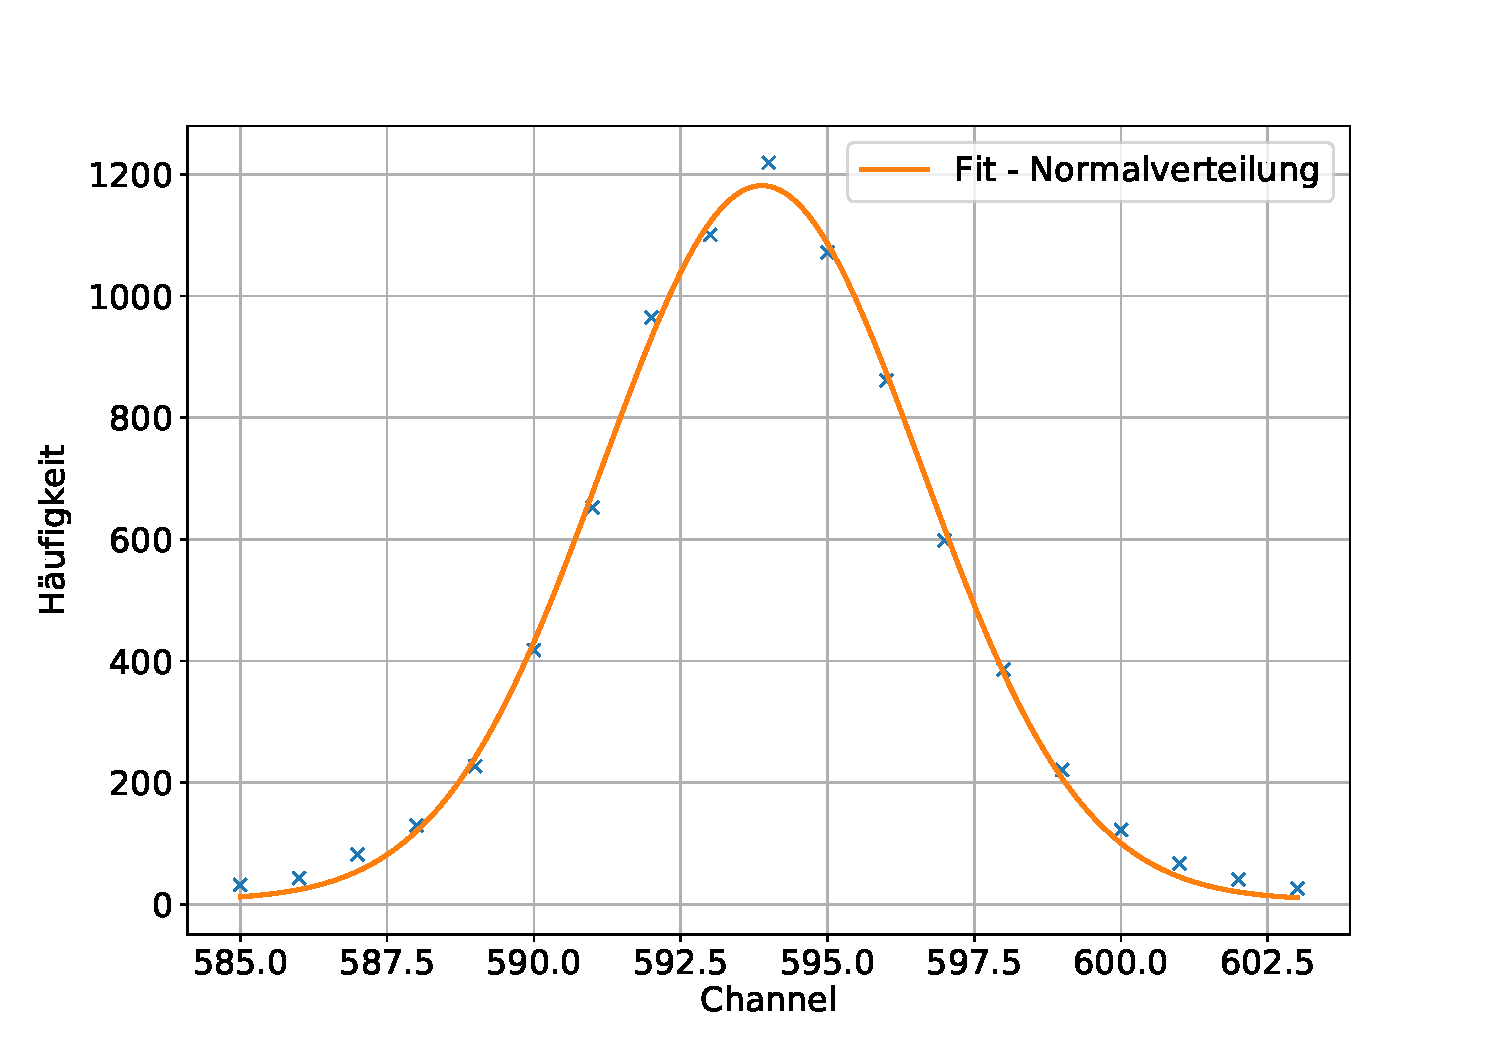
\includegraphics[width=0.8\textwidth]{content/images/einzelnergaussfit_0.pdf}
  \caption{Vergrößerung des ersten Peaks mit Ausgleichsfunktion einer Gaußkurve zur Veranschaulichung der Gaußpeaks.}
  \label{fig:einzelnergaussfit_0}
\end{figure}
Die Inhalte der Peaks werden durch Aufsummation der Counts im jeweiligen angepassten Datenbereich berechnet.
Die Ergebnisse zu den jeweiligen Peaks sind in Tabelle \ref{tab:vw} notiert.
\begin{table}[h!]
  \centering
  \caption{Parameter zur Berechnung der Vollenergienachweiswahrscheinlichkeit anhand eines $^{152}\symup{Eu}$-Spektrums. Weitere verwendete Größen sind: \\ $A=\SI{1545(29)}{\per \second}$, $\frac{\Omega}{4 \pi} = \SI{0.0069}{sr}$, $T=\SI{2134}{s}$.}
  \label{tab:vw}
  \begin{tabular}{ r  r  r  r  r  r  }
    \bottomrule
              $E_{\gamma}$ / keV \cite{nucleide} & $P$ \cite{nucleide}   & $P_{\text{Peakinhalt}}$    & Q in $10^{-3}$            \\ % & $a$                              &      $\mu$                         & $\sigma$                         & $b$                              \\
    \midrule
                $\SI{121.7817}{\nothing}$        & $\SI{28.41}{\nothing}$& $\SI{8233 (91)}{\nothing}$ & $\SI{12.70 (24)}{\nothing}$            \\ % & $\SI{54643  (699)}{a}$  & $\SI{593.88 (0.02}}{a}$      & $\SI{2.72080278 (0.02096791)}{a}$  & $\SI{6.65464370 (0.155416486)}{a}$ \\
                $\SI{244.6974}{\nothing}$        & $\SI{ 7.55}{\nothing}$& $\SI{1515 (39)}{\nothing}$ & $\SI{ 8.79 (16)}{\nothing}$            \\ % & $\SI{10583 (1892)}{a}$  & $\SI{1186.58105 (0.33278)}{a}$       & $\SI{3.08985566 (0.33289872)}{a}$  & $\SI{7.46589080 (0.347744578)}{a}$ \\
                $\SI{344.2785}{\nothing}$        & $\SI{26.59}{\nothing}$& $\SI{3152 (56)}{\nothing}$ & $\SI{ 5.19 (10)}{\nothing}$            \\ % & $\SI{25365 (2038)}{a}$  & $\SI{1666.69026 (0.16131)}{a}$       & $\SI{3.33202744 (0.16137103)}{a}$  & $\SI{7.26196957 (0.334424003)}{a}$ \\
                $\SI{411.1165}{\nothing}$        & $\SI{2.238}{\nothing}$& $\SI{ 324 (18)}{\nothing}$ & $\SI{ 6.34 (12)}{\nothing}$            \\ % & $\SI{ 1320 (1390)}{a}$  & $\SI{1989.13968353 (1.58221965)}{a}$ & $\SI{2.49555989 (1.58264810)}{a}$  & $\SI{7.60693051 (0.351207638)}{a}$ \\
                $\SI{ 443.965}{\nothing}$        & $\SI{ 2.80}{\nothing}$& $\SI{ 367 (19)}{\nothing}$ & $\SI{ 5.74 (11)}{\nothing}$            \\ % & $\SI{ 1839 (1909)}{a}$  & $\SI{2147.41246865 (1.92603485)}{a}$ & $\SI{3.08211825 (1.92667938)}{a}$  & $\SI{7.60363599 (0.351271659)}{a}$ \\
                $\SI{778.9045}{\nothing}$        & $\SI{12.97}{\nothing}$& $\SI{ 741 (27)}{\nothing}$ & $\SI{ 2.50  (5)}{\nothing}$            \\ % & $\SI{ 6632 (3679)}{a}$  & $\SI{3763.60345 (1.60581703)}{a}$    & $\SI{4.79839449 (1.60665042)}{a}$  & $\SI{7.56537596 (0.351196062)}{a}$ \\
                $\SI{ 964.079}{\nothing}$        & $\SI{14.50}{\nothing}$& $\SI{ 596 (24)}{\nothing}$ & $\SI{ 1.80 (33)}{\nothing}$            \\ % & $\SI{ 5190 (4028)}{a}$  & $\SI{4656.71298 (2.39004332)}{a}$    & $\SI{5.10185800 (2.39136059)}{a}$  & $\SI{7.58314830 (0.351416184)}{a}$ \\
                $\SI{1085.837}{\nothing}$        & $\SI{10.13}{\nothing}$& $\SI{ 403 (20)}{\nothing}$ & $\SI{ 1.74 (32)}{\nothing}$            \\ % & $\SI{ 2217 (3342)}{a}$  & $\SI{5244.21808 (4.04291370)}{a}$    & $\SI{4.46961617 (4.04488016)}{a}$  & $\SI{7.60853282 (0.351488937)}{a}$ \\
                $\SI{1112.076}{\nothing}$        & $\SI{13.41}{\nothing}$& $\SI{ 502 (22)}{\nothing}$ & $\SI{ 1.64 (30)}{\nothing}$            \\ % & $\SI{ 3576 (3677)}{a}$  & $\SI{5370.46910 (2.93022325)}{a}$    & $\SI{4.74729689 (2.93174255)}{a}$  & $\SI{7.59600458 (0.351461227)}{a}$ \\
                $\SI{1408.013}{\nothing}$        & $\SI{20.85}{\nothing}$& $\SI{ 586 (24)}{\nothing}$ & $\SI{ 1.23 (23)}{\nothing}$            \\ % & $\SI{ 5304 (5433)}{a}$  & $\SI{6798.07269 (4)}{a}$    & $\SI{6.16476521 (3.79392683)}{a}$  & $\SI{7.59078829 (0.351623258)}{a}$ \\
    \toprule
  \end{tabular}
\end{table}
%                                &  \scriptsize{$\sfrac{mN}{sm}{a}$}            &  \scriptsize{$\sfrac{mN}{m}{a}$}          &  \scriptsize{$\sfrac{mN}{m}{a}$} &  \scriptsize{$\sfrac{mN}{m}{a}$} & \scriptsize{$\sfrac{mN}{m}{a}$} \\ \hline \hline
%    \rowcolor{Lightgray} \multicolumn{7}{|c|}{Referenzen}\\ \hline
%        \multirow{2}{*}{\ce{C3F8}}  & 1  & $\SI{ 1.3396 \pm 0.0202 e-3}{\nothing}{a}$  &  $\SI{ -0.5415 \pm 0.0558 }{\nothing} $  &  $\SI{ 0.00 }{\nothing}{a}$      &  $\SI{ 5.72 }{\nothing}{a}$   & $\SI{ 5.72 }{\nothing}{a}$    \\

Nun wird $Q$ gegen die Energie $E$ des jeweiligen Peaks aufgetragen.
Es wird eine Ausgleichsrechnung der Form $Q=a E^{b} + c$ durchgeführt.
\begin{figure}[h!]
  \centering
  \includegraphics[width=0.8\textwidth]{content/images/vollenergienachweiswahrscheinlichkeit.pdf}
  \caption{Ausgleichsrechnung zur Bestimmung der Vollenergienachweiswahrscheinlichkeit $Q$.
  Die Fehlerbereiche verschwinden hinter den Datenpunkten und sind zur Übersichtlichkeit nicht aufgeführt.}
  \label{fig:vw}
\end{figure}
Die Parameter der Ausgleichsrechnung betragen:
\begin{align*}
	a = \SI{0.113 (55)}{\frac{1}{\kilo \electronvolt}}, && b = \SI{-0.36 (17)}{\nothing}, && c = \SI{-0.0077 (59)}{\nothing}.
\end{align*}

%mit $t = \SI{605484000 (54000)}{s}$
%und $T_{\sfrac{1}{2}} = \SI{426.7 (5) e+06}{s}$ \cite{nucleide}
%\begin{equation}
%	A = A_{0} \exp{\left( - \frac{\ln{(2))}}{T_{\sfrac{1}{2}}} t \right)} = \SI{1545(29)}{\per \second}
%	\label{result:aktivität}
%\end{equation}
%mit $r=\SI{22.5e-03}{m}$
%und $h = \SI{80e-03}{m}$
%\begin{align*}
%	\frac{r}{h} = \tan{( \varphi / 2 )} \Leftrightarrow \varphi = 2 \arctan{(\frac{r}{h})} \\
%	\frac{\Omega}{4 \pi} = \sin^2{\frac{\varphi}{2 \cdot 4}} =  \sin^2{ \left( \frac{1}{4} \arctan{(r/h)} \right)} = \SI{0.0069}{sr}
%	\label{result:raumwinkel}
%\end{align*}
%und
%\begin{equation}
%	Q = \frac{4 \pi}{\Omega} \frac{N_{\text{Peakinhalt}}}{ A T P_{E_{\gamma}}}
%\end{equation}

%\begin{figure}[h!]
%  \centering
%  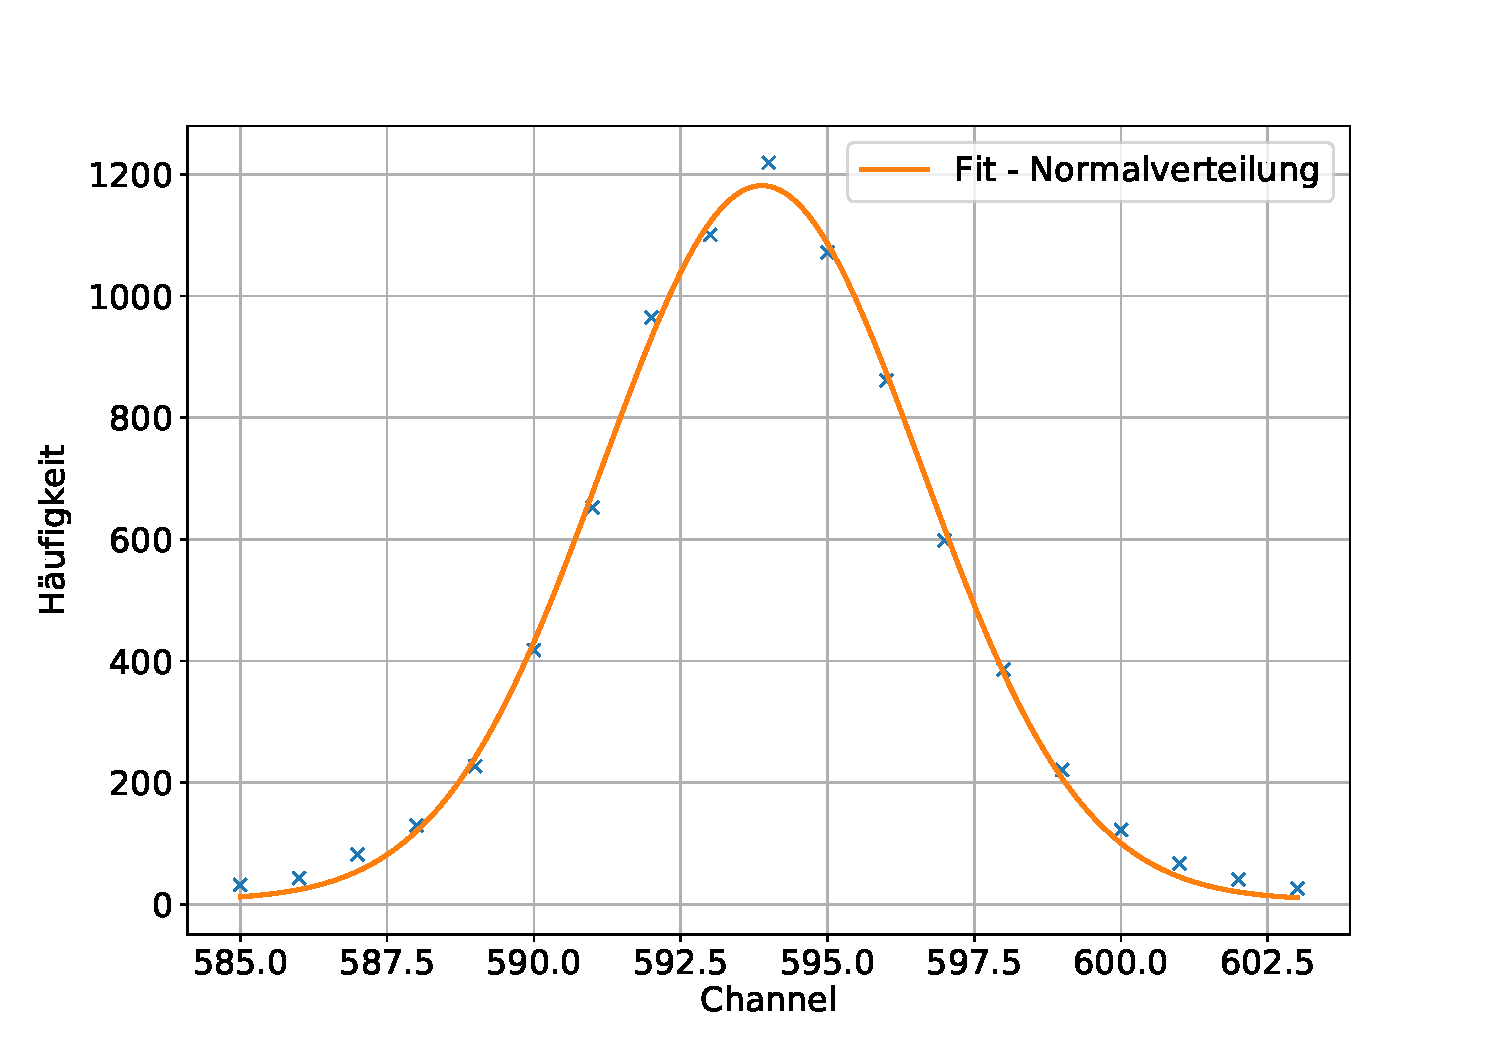
\includegraphics[width=0.8\textwidth]{content/images/einzelnergaussfit_0.pdf}
%  \caption{Vergrößerung des ersten Peaks mit Ausgleichsfunktion einer Gaußkurve zur Veranschaulichung der Gaußpeaks.}
%  \label{fig:vw}
%\end{figure}

%\begin{table}[h!]
  \centering
  \caption{Parameter zur Berechnung der Vollenergienachweiswahrscheinlichkeit anhand eines $^{152}\symup{Eu}$-Spektrums. Weitere verwendete Größen sind: \\ $A=\SI{1545(29)}{\per \second}$, $\frac{\Omega}{4 \pi} = \SI{0.0069}{sr}$, $T=\SI{2134}{s}$.}
  \label{tab:vw}
  \begin{tabular}{ r  r  r  r  r  r  }
    \bottomrule
              $E_{\gamma}$ / keV \cite{nucleide} & $P$ \cite{nucleide}   & $P_{\text{Peakinhalt}}$    & Q in $10^{-3}$            \\ % & $a$                              &      $\mu$                         & $\sigma$                         & $b$                              \\
    \midrule
                $\SI{121.7817}{\nothing}$        & $\SI{28.41}{\nothing}$& $\SI{8233 (91)}{\nothing}$ & $\SI{12.70 (24)}{\nothing}$            \\ % & $\SI{54643  (699)}{a}$  & $\SI{593.88 (0.02}}{a}$      & $\SI{2.72080278 (0.02096791)}{a}$  & $\SI{6.65464370 (0.155416486)}{a}$ \\
                $\SI{244.6974}{\nothing}$        & $\SI{ 7.55}{\nothing}$& $\SI{1515 (39)}{\nothing}$ & $\SI{ 8.79 (16)}{\nothing}$            \\ % & $\SI{10583 (1892)}{a}$  & $\SI{1186.58105 (0.33278)}{a}$       & $\SI{3.08985566 (0.33289872)}{a}$  & $\SI{7.46589080 (0.347744578)}{a}$ \\
                $\SI{344.2785}{\nothing}$        & $\SI{26.59}{\nothing}$& $\SI{3152 (56)}{\nothing}$ & $\SI{ 5.19 (10)}{\nothing}$            \\ % & $\SI{25365 (2038)}{a}$  & $\SI{1666.69026 (0.16131)}{a}$       & $\SI{3.33202744 (0.16137103)}{a}$  & $\SI{7.26196957 (0.334424003)}{a}$ \\
                $\SI{411.1165}{\nothing}$        & $\SI{2.238}{\nothing}$& $\SI{ 324 (18)}{\nothing}$ & $\SI{ 6.34 (12)}{\nothing}$            \\ % & $\SI{ 1320 (1390)}{a}$  & $\SI{1989.13968353 (1.58221965)}{a}$ & $\SI{2.49555989 (1.58264810)}{a}$  & $\SI{7.60693051 (0.351207638)}{a}$ \\
                $\SI{ 443.965}{\nothing}$        & $\SI{ 2.80}{\nothing}$& $\SI{ 367 (19)}{\nothing}$ & $\SI{ 5.74 (11)}{\nothing}$            \\ % & $\SI{ 1839 (1909)}{a}$  & $\SI{2147.41246865 (1.92603485)}{a}$ & $\SI{3.08211825 (1.92667938)}{a}$  & $\SI{7.60363599 (0.351271659)}{a}$ \\
                $\SI{778.9045}{\nothing}$        & $\SI{12.97}{\nothing}$& $\SI{ 741 (27)}{\nothing}$ & $\SI{ 2.50  (5)}{\nothing}$            \\ % & $\SI{ 6632 (3679)}{a}$  & $\SI{3763.60345 (1.60581703)}{a}$    & $\SI{4.79839449 (1.60665042)}{a}$  & $\SI{7.56537596 (0.351196062)}{a}$ \\
                $\SI{ 964.079}{\nothing}$        & $\SI{14.50}{\nothing}$& $\SI{ 596 (24)}{\nothing}$ & $\SI{ 1.80 (33)}{\nothing}$            \\ % & $\SI{ 5190 (4028)}{a}$  & $\SI{4656.71298 (2.39004332)}{a}$    & $\SI{5.10185800 (2.39136059)}{a}$  & $\SI{7.58314830 (0.351416184)}{a}$ \\
                $\SI{1085.837}{\nothing}$        & $\SI{10.13}{\nothing}$& $\SI{ 403 (20)}{\nothing}$ & $\SI{ 1.74 (32)}{\nothing}$            \\ % & $\SI{ 2217 (3342)}{a}$  & $\SI{5244.21808 (4.04291370)}{a}$    & $\SI{4.46961617 (4.04488016)}{a}$  & $\SI{7.60853282 (0.351488937)}{a}$ \\
                $\SI{1112.076}{\nothing}$        & $\SI{13.41}{\nothing}$& $\SI{ 502 (22)}{\nothing}$ & $\SI{ 1.64 (30)}{\nothing}$            \\ % & $\SI{ 3576 (3677)}{a}$  & $\SI{5370.46910 (2.93022325)}{a}$    & $\SI{4.74729689 (2.93174255)}{a}$  & $\SI{7.59600458 (0.351461227)}{a}$ \\
                $\SI{1408.013}{\nothing}$        & $\SI{20.85}{\nothing}$& $\SI{ 586 (24)}{\nothing}$ & $\SI{ 1.23 (23)}{\nothing}$            \\ % & $\SI{ 5304 (5433)}{a}$  & $\SI{6798.07269 (4)}{a}$    & $\SI{6.16476521 (3.79392683)}{a}$  & $\SI{7.59078829 (0.351623258)}{a}$ \\
    \toprule
  \end{tabular}
\end{table}
%                                &  \scriptsize{$\sfrac{mN}{sm}{a}$}            &  \scriptsize{$\sfrac{mN}{m}{a}$}          &  \scriptsize{$\sfrac{mN}{m}{a}$} &  \scriptsize{$\sfrac{mN}{m}{a}$} & \scriptsize{$\sfrac{mN}{m}{a}$} \\ \hline \hline
%    \rowcolor{Lightgray} \multicolumn{7}{|c|}{Referenzen}\\ \hline
%        \multirow{2}{*}{\ce{C3F8}}  & 1  & $\SI{ 1.3396 \pm 0.0202 e-3}{\nothing}{a}$  &  $\SI{ -0.5415 \pm 0.0558 }{\nothing} $  &  $\SI{ 0.00 }{\nothing}{a}$      &  $\SI{ 5.72 }{\nothing}{a}$   & $\SI{ 5.72 }{\nothing}{a}$    \\


%\begin{itemize}
%	\item Unterteilung der Daten in die Abschnitte um die Peaks (channel und counts werden passend abgeschnitten)
%	\item Über die Peaks wird eine Gaußkurve gelegt $f (x) = \frac{a}{\sqrt{2 \pi \sigma^2}} \exp{\left( - \frac{(x-\mu)^2}{2 \sigma^2} \right)}+b$
%	\item Klappt bei den meisten Peaks ganz gut, aber manchmal ist der Fehler des Parameters $a$ größer als a :|
%	\item Alternative für Inhalt: Aufsummation der Counts in den jeweiligen Intervallen, Fehler über den Poisson-Fehler ($N \pm \sqrt{N}$)
%	\item $Q$ berechnet mit $A$ aus \eqref{result:aktivität}, $\sfrac{\Omega}{4 \pi}$ aus \eqref{result:raumwinkel},
%	gesamte Messzeit $T=\SI{2134}{s}$, Emissionswahrscheinlichkeit $P_{E_{\gamma}}$ aus \cite{nucleide}, Peakinhalt $N_{\text{Peakinhalt}}$
%	\item $Q$ gegen $E$ aufgetragen, $Q=a E^{b} + c$, Parameter:
%\end{itemize}
%\begin{align*}
%	a = \SI{0.113 (55)}{\frac{1}{J}}, && b = \SI{-0.36 (17)}{\nothing}, && c = \SI{-0.0077 (59)}{\nothing}
%\end{align*}

%\begin{figure}[h!]
%  \centering
%  \includegraphics[width=0.8\textwidth]{content/images/vollenergienachweiswahrscheinlichkeit.pdf}
%  \caption{Ausgleichsrechnung zur Bestimmung der Vollenergienachweiswahrscheinlichkeit $Q$.
%  Die Fehlerbereiche verschwinden hinter den Datenpunkten und sind zur Übersichtlichkeit nicht aufgeführt.}
%  \label{fig:vw}
%\end{figure}

\FloatBarrier
\subsection{Monochromatisches $^{137}\symup{Cs}$-Spektrum}
In Abbildung \ref{fig:cs_spectrum} ist das volle Spektrum des $^{137}\symup{Cs}$-Strahlers abgebildet.
\begin{figure}[h!]
  \centering
  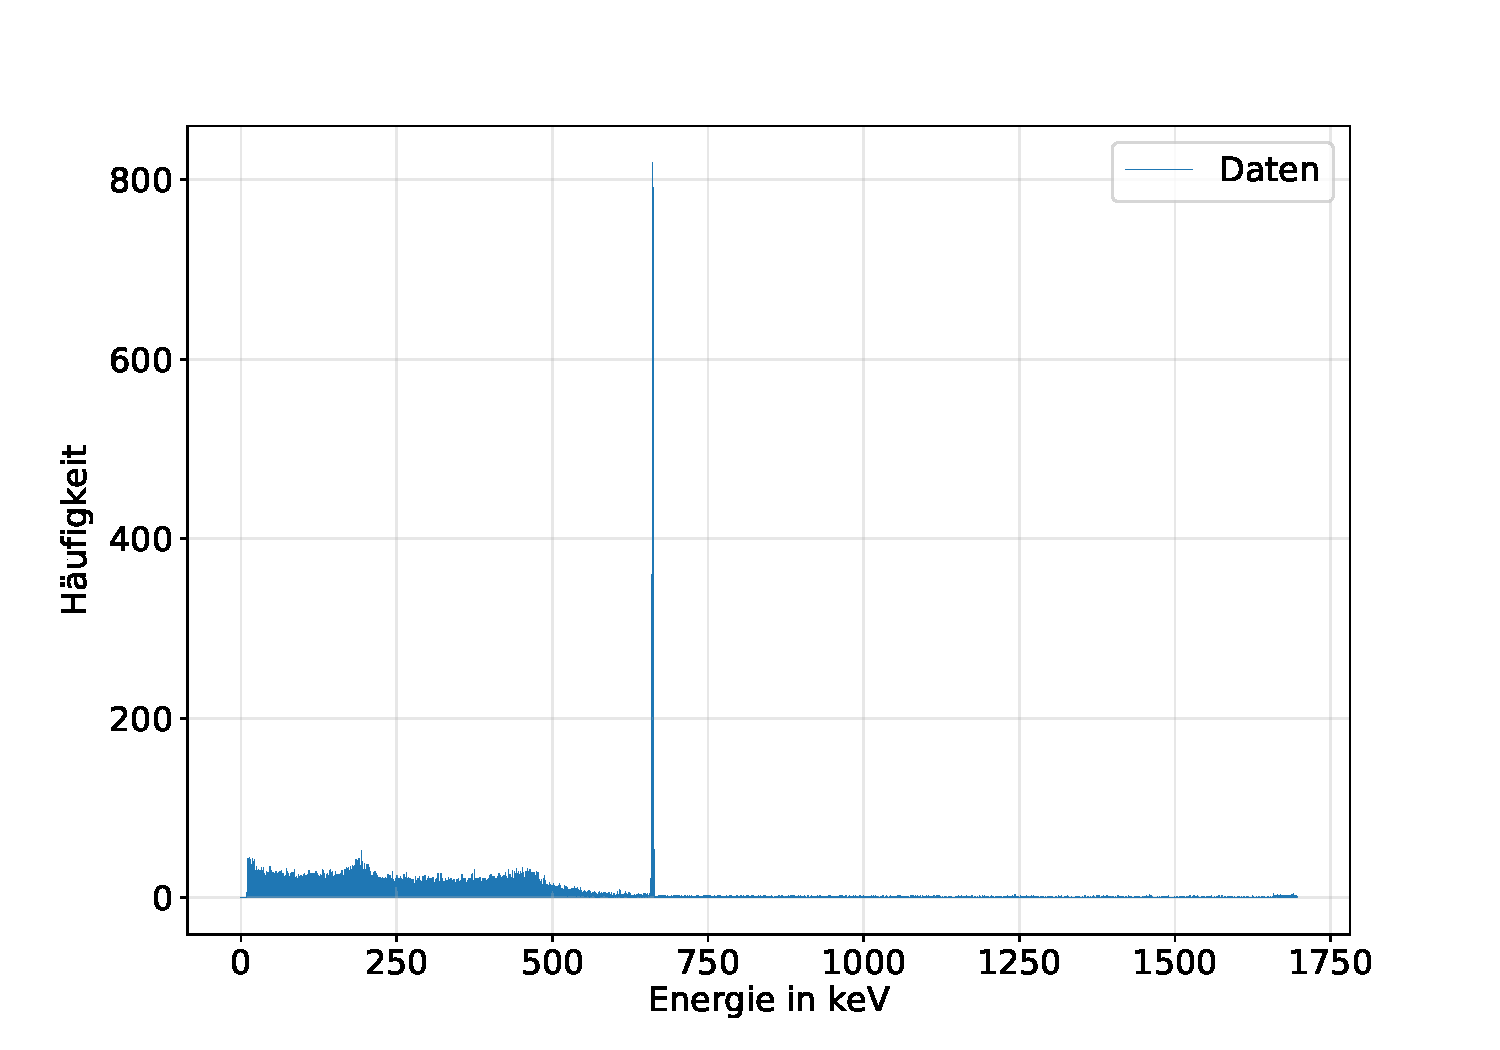
\includegraphics[width=0.8\textwidth]{content/images/caesium_vollesspektrum.pdf}
  \caption{Volles aufgenommenes Spektrum des $^{137}\symup{Cs}$-Strahlers.}
  \label{fig:cs_spectrum}
\end{figure}
Der Photopeak wird über eine Peak-Picking-Funktion ermittelt.
Dieser ist vergrößert in Abbildung \ref{fig:cs_photopeak} abgebildet.
\begin{figure}[h!]
  \centering
  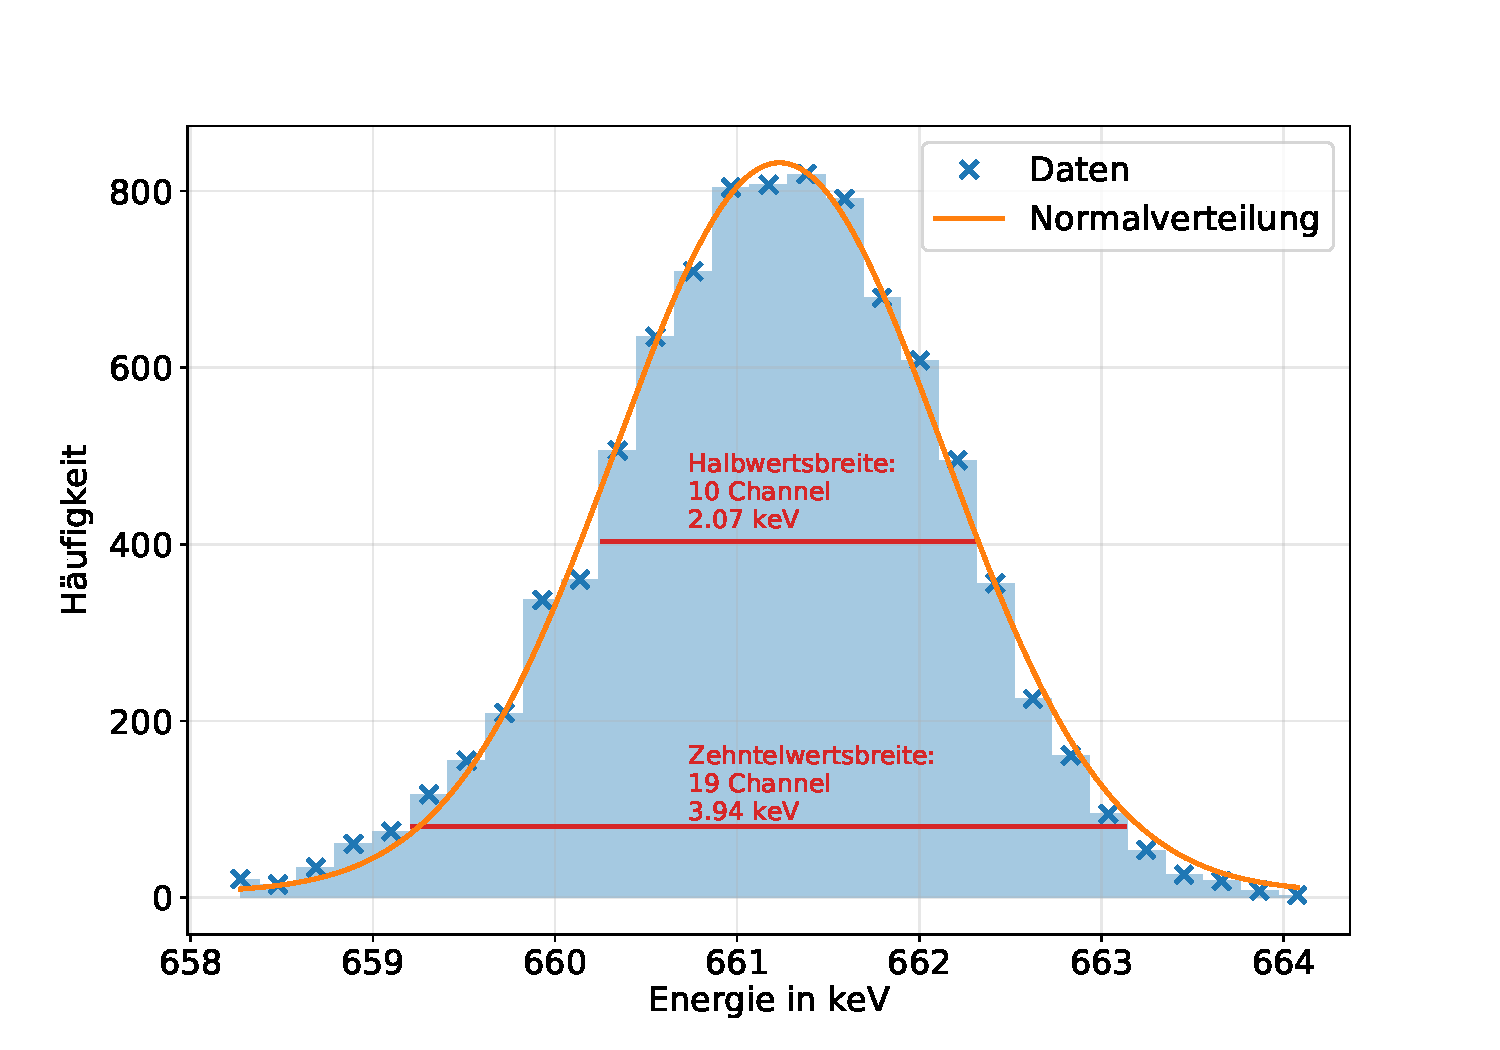
\includegraphics[width=0.8\textwidth]{content/images/caesium_peak_1.pdf}
  \caption{Vergrößerter Photopeak des $^{137}\symup{Cs}$-Strahlers.}
  \label{fig:cs_photopeak}
\end{figure}
An den Peak wird eine Gaußverteilung nach
\begin{equation*}
	f(E) = \frac{a}{\sqrt{2 \pi \sigma^2}} \, \exp{\left( - \frac{(E-\mu)^2}{2 \sigma^2} \right)} + b
\end{equation*}
gefittet.
Hierzu wird der augewertete Datenbereich angepasst.
Die Parameter der Ausgleichsrechnung ergeben sich zu
\begin{align*}
	\mu = \SI{661.2327 (51)}{\kilo \electronvolt}, 	&& \sigma = \SI{0.9023 (51)}{\kilo \electronvolt}, \\
	 a = \SI{1868 (9)}{\kilo \electronvolt^2}, 		&& b = \SI{6.1 (1)}{\kilo \electronvolt}.
\end{align*}
Für den Inhalt des Photopeaks werden die Counts im geplotteten Bereich aufsummiert.
Der Inhalt beträgt:
\begin{equation*}
	N_{\text{Peak}} = \SI{9174 (96)}{\nothing}.
\end{equation*}
Die Halbwertsbreite (FWHM) und die Zehntelwertsbreite (FWTM) werden zu folgenden Daten ausgemessen, indem die Energie bei der Hälfte bzw einem Zehntel der Counts aus den Messdaten bestimmt wird:
\begin{align*}
	\text{FWHM}_{\text{Daten}} && = && \SI{2.07}{\kilo \electronvolt}\\
	\text{FWTM}_{\text{Daten}} && = && \SI{3.94}{\kilo \electronvolt}\\
	\frac{ \text{FWHM}_{\text{Daten}} }{ \text{FWTM}_{\text{Daten}} } && = && \SI{0.53}{\nothing}. \\
\end{align*}
Aus der Standardabweichung $\sigma$ lässt sich ein Vergleichswert passend zur gefitteten Gaußverteilung finden:
\begin{align*}
	\text{FWHM}_{\text{Fit}} && = && 2 \sigma \, \sqrt{2 \ln{(2)}}    = \SI{2.13}{\kilo \electronvolt}\\
	\text{FWTM}_{\text{Fit}} && = && 2 \sigma \, \sqrt{2 \ln{(10)}}  = \SI{3.87}{\kilo \electronvolt}\\
	\frac{ \text{FWHM}_{\text{Fit}} }{ \text{FWTM}_{\text{Fit}} } && = && \SI{0.55}{\nothing}. \\
\end{align*}
In Abbildung \ref{fig:cs_kontinuum} ist das Compton-Kontinuum des Spektrums vergrößert dargestellt.
\begin{figure}[h!]
  \centering
  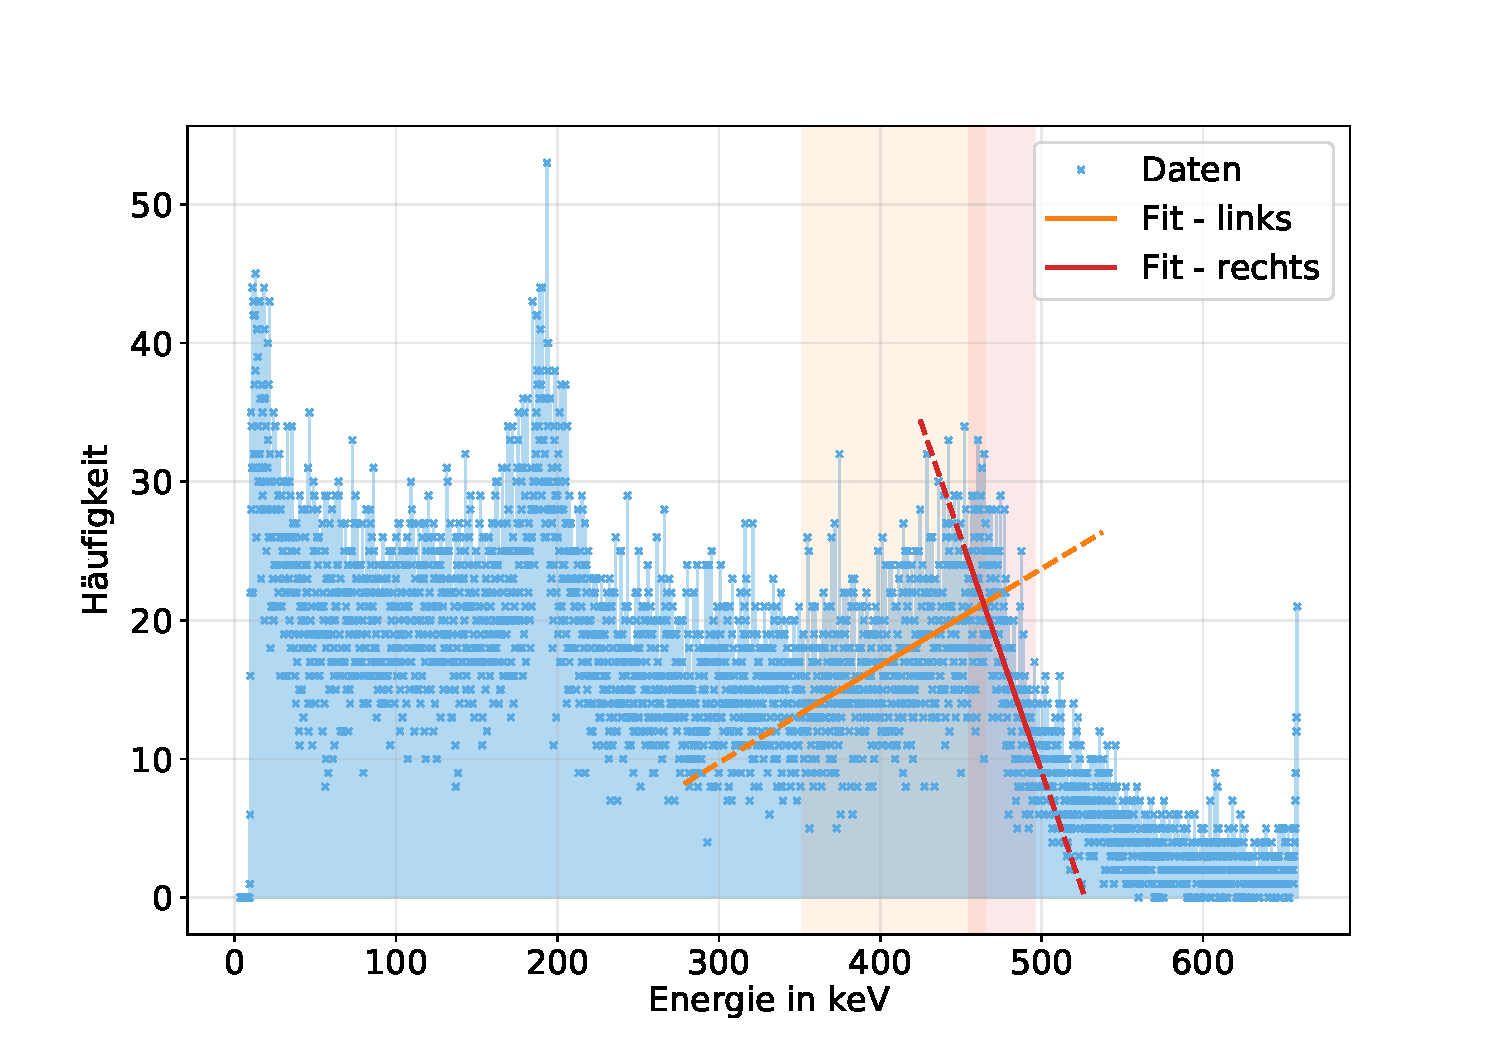
\includegraphics[width=0.8\textwidth]{content/images/caesium_kontinuum.pdf}
  \caption{Vergrößertes Compton-Kontinuum des $^{137}\symup{Cs}$-Strahlers mit linearen Ausgleichsrechnungen zur Identifitkation der Lage der Compton-Kante.}
  \label{fig:cs_kontinuum}
\end{figure}
Über den Schnittpunkt zweier Ausgleichsgeraden der Form $y = a \cdot E + b$ wird die Lage der Compton-Kante angenähert.
Die Parameter der Geraden ergeben sich zu
\begin{align*}
	\text{links:}  && a & = & \SI{0.0699 (58)}{\frac{1}{\kilo \electronvolt}}, && b & = & \SI{-11.3 (24)}{\nothing}, \\
	\text{rechts:} && a & = & \SI{-0.152 (17)}{\frac{1}{\kilo \electronvolt}}, && b & = & \SI{ 89 (8)}{\nothing}. \\
\end{align*}
Der Schnittpunkt, entsprechend die Compton-Kante, liegt über Gleichsetzen der Geradengleichungen bei
\begin{equation*}
	E_{\text{CK, Data}} = \SI{450 (5)}{\kilo \electronvolt}.
\end{equation*}
Aus Gleichung \eqref{eq:compton_kante} folgt für die Compton-Kante folgender theoretischer Wert:
\begin{equation*}
	E_{\text{CK, Theo}} = \SI{477.3340 (28)}{\kilo \electronvolt}.
\end{equation*}
Der Inhalt des Compton-Kontinuums als Summation der betreffenden Kanalinhalte bis zur Compton-Kante beträgt
\begin{equation*}
	N_{\text{Kontinuum, komplett}} = \SI{40797}{\nothing}. % ohne Wirkungsquerschnitt verrechnet
\end{equation*}

Rückstreuung bei $\vartheta = \SI{90}{°}$:
\begin{equation}
    {E'}_{\!\gamma} = \frac{E_\gamma}{1 + \frac{E_\gamma}{m_e c^2} \left(1 - \cos\vartheta \right)} = \SI{242.1(11)}{\kilo \electronvolt}
    \label{eq:rückstreu}
\end{equation}
Wirkungsquerschnitt ($\varepsilon = E_\gamma / m c^2 << 1$, $\sigma_{Th} = \frac{1}{6 \pi \epsilon_0^2} \frac{e^4}{m_{e}^2 c^4}$):
\begin{equation}
    \sigma_{Co} \sim \frac{3}{4}\sigma_{Th} \left(1 - 2\varepsilon + \frac{26}{5}\varepsilon^2 \right).
\end{equation}
%
%Suche
%\begin{itemize}
%	\item Energie des Strahlers (Photo-Energie -> Gauss fitten? mu entspricht dann dem Channel und der Channel einer Energie)
%	\item Fit:
%	\begin{equation*}
%		f(x) = \frac{a}{\sqrt{2 \pi \sigma^2}} \, \exp{\left( - \frac{(x-\mu)^2}{2 \sigma^2} \right)} + b
%	\end{equation*}
%	\item Parameter
%	\begin{align*}
%		\mu = \SI{661.2327 (51)}{\kilo \electronvolt} && \sigma = \SI{0.9023 (51)}{\kilo \electronvolt} && a = \SI{1868 (9)}{\nothing} && b = \SI{6.1 (1)}{\nothing}
%	\end{align*}
%	\item Halbwertsbreite fitten
%	\item Zehntelwertsbreite fitten, $FWHM/FWTM(Theorie) = 0.5486620049392714$, in den Daten: $FWHM/FWTM = 0.5486620049392715$
%	\item
%	\begin{align*}
%		FWHM = 10 && FWTM = 19
%	\end{align*}
%	\item Comptonkante ausmessen, bei:
%	\begin{align*}
%		E = \SI{4.6 (4)e+02}{\kilo \electronvolt}
%	\end{align*}
%	\item
%	mit den Parametern
%	\begin{align*}
%		links   && rechts \\
%		a = \SI{0.0699 (58)}{\frac{1}{\kilo \electronvolt}} && a = \SI{ -0.337 (27)}{\frac{1}{\kilo \electronvolt}} \\
%		b = \SI{ -11.3 (24)}{\nothing} 						&& b = \SI{ 178 (13)}{\nothing} \\
%	\end{align*}
%	\item Theorie liegt bei
	Rückstreulinie ausmessen
	über Geradenschnittpunkt in Rückstreulinie
	Inhalte des Peaks und des Compton-Kontinuums ausmessen (aufsummieren, aaaaber... Anleitung!)
